% This file was created by tikzplotlib v0.9.4.
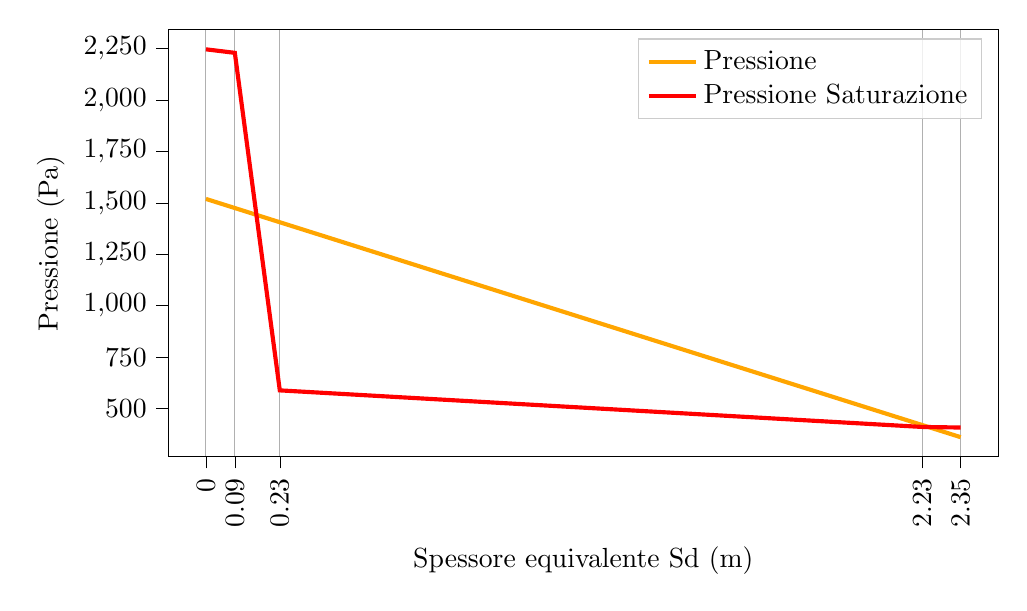
\begin{tikzpicture}

\definecolor{color0}{rgb}{1,0.647058823529412,0}

\begin{axis}[
	 ticklabel style={ 
 		 /pgf/number format/fixed, 
 		 /pgf/number format/precision=5
		}, 
scaled ticks=false,
height=7cm,
legend cell align={left},
legend style={fill opacity=0.8, draw opacity=1, text opacity=1, draw=white!80!black},
minor xtick={},
minor ytick={},
tick align=outside,
tick pos=left,
width=\textwidth,
x grid style={white!69.0196078431373!black},
xlabel={Spessore equivalente Sd (m)},
xmajorgrids,
xmin=-0.1175, xmax=2.4675,
xtick style={color=black},
xtick={0,0.09,0.23,2.23,2.35},
xticklabel style = {rotate=90.0},
y grid style={white!69.0196078431373!black},
ylabel={Pressione (Pa)},
ymin=266.815315862144, ymax=2340.26179765774,
ytick style={color=black},
ytick={250,500,750,1000,1250,1500,1750,2000,2250,2500}
]
\addplot [line width=1.5pt, color0]
table {%
0 1519.01824347152
0.09 1474.67101690856
0.23 1405.68644225507
2.23 420.192518633768
2.35 361.06288321649
};
\addlegendentry{Pressione}
\addplot [line width=1.5pt, red]
table {%
0 2246.0142303034
0.09 2228.8857975183
0.23 588.588856594798
2.23 410.858360238758
2.35 407.990247749789
};
\addlegendentry{Pressione Saturazione}
\end{axis}

\end{tikzpicture}
